%loading the preamble with LaTeX commands/classes
% Document class and language setting
\documentclass[12pt, oneside, paper=A4, DIV=15, BCOR=0mm, abstract=true, headings=small]{scrartcl}
\usepackage[english]{babel} % Changed from ngerman
\usepackage[utf8]{inputenc}

% Font
%LModern
\usepackage{lmodern}
%Libertine
%\usepackage{libertinus}
%\usepackage{libertinust1math}

\usepackage[T1]{fontenc}

% Control headers and footers with scrlayer-scrpage
% Separator line top and bottom
\usepackage[headsepline, footsepline]{scrlayer-scrpage}

% Math, symbols, unit representation, chemistry
\usepackage{amsmath}
\usepackage{amsxtra}
\usepackage{eurosym}
\usepackage{siunitx}  
\sisetup{locale=US} % Changed from DE
\usepackage[version=4]{mhchem}

% Typography
\usepackage[auto]{microtype}
\clubpenalty = 10000
\widowpenalty = 10000
\displaywidowpenalty = 10000

% Inclusion of images, tables, pdf pages, source code
\usepackage{graphicx}
\usepackage{multirow, multicol, booktabs}
\usepackage{threeparttable}
\usepackage{longtable}
\usepackage{rotating}
\usepackage{ltablex}
\usepackage{subfig}
\captionsetup[subtable]{position=top}
\usepackage{pdfpages}
\usepackage{listings}
\usepackage{placeins}

% Display of URL
\usepackage{url}
\urlstyle{same}

% Footnotes, also for tables
\usepackage{footnote}
\makesavenoteenv{tabular} 

% Packages for control and review
\usepackage{todonotes}
\usepackage{blindtext}

% Representation of bibliography entries
\usepackage[
backend=biber,
style=ieee,
citestyle=numeric-comp,
maxbibnames=2,
firstinits=true
]{biblatex}

\renewcommand*{\labelnamepunct}{\addcolon\addspace}

% Storage location of the bibliography (*.bib file)
\addbibresource{bibliography.bib}

% Footnotes
% Mark in the footnote itself neither superscripted nor set smaller
% \deffootnote{1em}{1em}{\thefootnotemark\ }
% left-aligned footnote markers
\deffootnote{1.5em}{1em}{%
  \makebox[1.5em][l]{\thefootnotemark}%
}

% Do not break footnotes
\interfootnotelinepenalty=10000

% Design of image captions and table headings as well as title page information
\addtokomafont{caption}{\small}
\setkomafont{captionlabel}{\sffamily\bfseries}
\setkomafont{subject}{\Large\bfseries}
\setkomafont{author}{\normalfont}
\setkomafont{date}{\normalfont}
\setkomafont{publishers}{\normalfont}


\makeatletter
% \renewcommand{\l@section}{\@dottedtocline{1}{0em}{0em}}
% \renewcommand{\l@subsection}{\@dottedtocline{2}{4ex}{3.6em}}
% \g@addto@macro{\@afterheading}{\vspace{-0.25\baselineskip}}
\renewcommand{\l@section}{\@dottedtocline{1}{0ex}{1.8em}}
\renewcommand{\l@subsection}{\@dottedtocline{2}{1.8em}{2.7em}}
% \g@addto@macro{\@afterheading}{\vspace{-0.25\baselineskip}}
\makeatother


\renewcaptionname{english}{\figurename}{Fig.} % Changed from ngerman and Abb.
\renewcaptionname{english}{\tablename}{Tab.}  % Changed from ngerman

% Table environments with font size 10 and 7
\newenvironment{tabular10}{%
  \fontsize{10}{12}\selectfont\tabular
}{%
  \endtabular
}

\newenvironment{tabular7}{%
  \fontsize{7}{12}\selectfont\tabular
}{%
  \endtabular
}

% Links and references, pdf settings
% Update information if necessary!
\usepackage[
pdftitle={Final Report}, % Translated from Abschlussmain
pdfsubject={},
pdfauthor={},
pdfkeywords={},  
% Do not frame links
hidelinks
]{hyperref}
\usepackage[english]{cleveref} % Changed from german


\begin{document}
\def\VARcompany{RAPPORT INTERMÉDIAIRE}

\def\VARtitle{Projet 7 Wonders - Groupe A}

\def\VARdate{Novembre 07, 2025}

\begin{titlepage}

%Headers and footers
\pagestyle{scrheadings}
\clearscrheadfoot

	\centering
	\pagenumbering{gobble} % This ensures this page has NO page number
	
	% 1. Logo
	
\includegraphics[width=1\textwidth]{UCA-Logo-2niveaux-RVB.jpg}
	
	\vspace{3em}
	
	% 2. University Name
	{\Large \textbf{\VARcompany}\par}
	
	\vspace{3em}
	
	% 3. First Line
	\rule{\textwidth}{1pt}
	\vspace{0em}
	
	% 4. Title 
	% Uses the \VARort variable from your main.tex
	{\Huge \textbf{\VARtitle}\par} 
	
	\vspace{1em}
	% 5. Second Line
	\rule{\textwidth}{1pt}
	
	\vspace{5em} % Pushes the block down
	
	% 6. Members Block
	\noindent % Prevents indentation
	\begin{minipage}[t]{0.45\textwidth}
		\textbf{Membres :}\\
		BOUTRIK Alexandre\\
		DIALLO Elhadj Oumar\\
		GHILANE EL HASSANI Abdelouarite\\
		MANILIUC David\\
		LANDOULSI Aziz\\
		RAHMOUNI Mohamed Khalil
	\end{minipage}
	\hfill % Pushes the next minipage to the right
	\begin{minipage}[t]{0.25\textwidth}
		\textbf{Enseignant :}\\
		DONATI Leo
	\end{minipage}
	
	\vfill % Pushes the date to the bottom
	
	% 7. Date
	{\large \VARdate\par}
	
\end{titlepage}
%global setting for source code display with listings
\lstset{basicstyle=\scriptsize\ttfamily,language={[LaTeX]TeX}}

%Arabic page numbering
\pagenumbering{arabic}

%Title
%\input{00a_titelei}
%Abstract
%\input{00b_abstract}
%Table of contents
\setcounter{tocdepth}{2}
\renewcommand{\contentsname}{Sommaire}
\tableofcontents

%Start of chapters
\section{Introduction}
\label{sec:introduction}

Ce rapport intermédiaire présente l'état d'avancement du Projet Informatique 7 Wonders. L'objectif est d'analyser la solution actuellement mise en œuvre pour le jeu, en détaillant son architecture , sa modélisation , et sa conception logicielle. Ce document abordera également les points forts et les axes d'amélioration identifiés à ce stade du développement
\section{Architecture}
\label{sec:architecture}

Cette section présente la structure globale du projet. L’architecture a été conçue de manière à favoriser la maintenabilité, la modularité et la testabilité du système, tout en demeurant cohérente avec les principes de conception orientée objet.

\subsection{Représentation Générale}
\label{sec:diagram-activity}

\FloatBarrier
\begin{figure}[h]
	\centering
	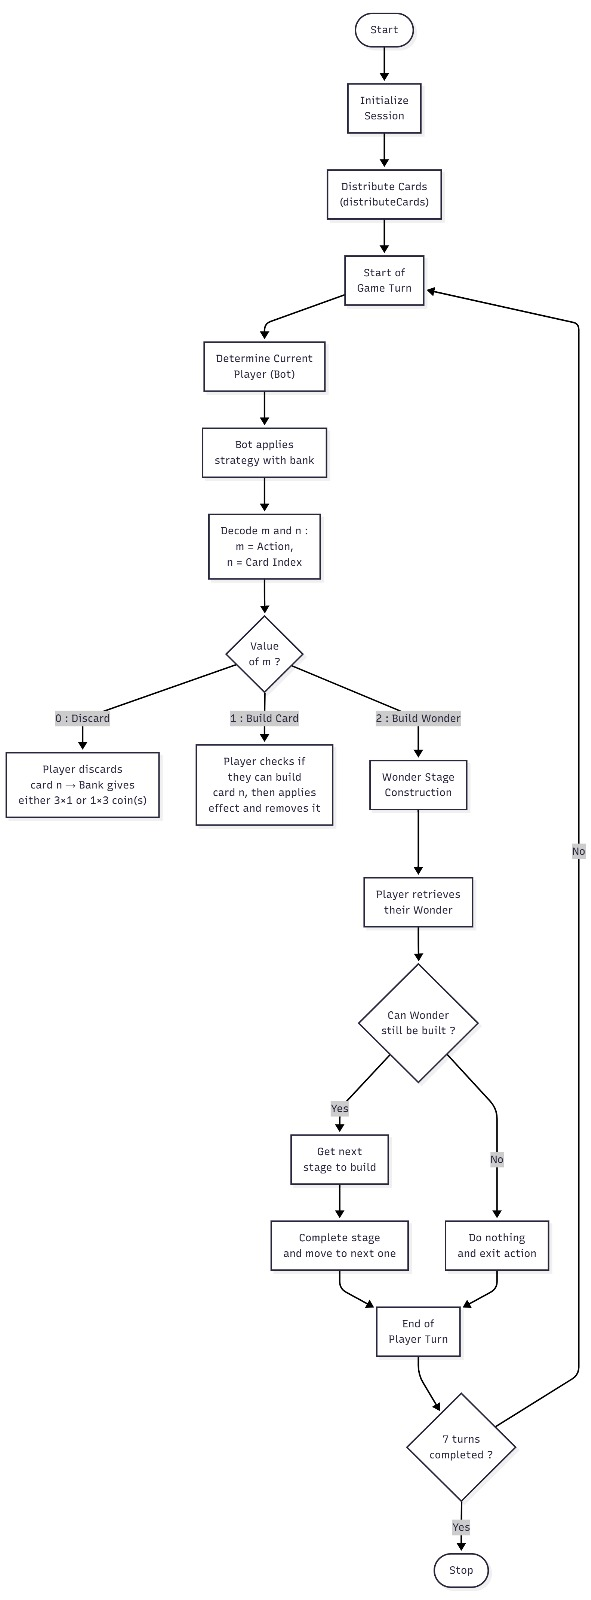
\includegraphics[width=0.5\textwidth]{activity.jpg}
	\caption{Diagramme d'activié}
	\label{fig:my-screenshot}
\end{figure}
\FloatBarrier

\subsection{Les Fonctionnalités Traitées}
\label{sec:functionalities}

Cette sous-section présente les fonctionnalités actuellement intégrées au projet, notamment l’intégration des modules Maven, la configuration de la suite de tests et l’état de l'implémentation des mécaniques de jeu.

\subsubsection{Modules Maven}
\label{sec:maven}

Le projet repose sur plusieurs modules Maven essentiels au bon déroulement du développement. Pour les tests unitaires, JUnit et Mockito (pour la création d’objets simulés) sont utilisés conjointement afin de tester les composants de manière isolée. Parallèlement, le plugin Maven Failsafe est configuré pour prendre en charge les tests d'intégration.

Spotless assure une homogénéité du style de code en appliquant des règles de formatage automatisées afin d'éviter les conflits de merge inutiles. JaCoCo est employé pour mesurer la couverture des tests et produire des rapports détaillés, ce qui permet d’évaluer la fiabilité des parties testées du code. Enfin, JavaDoc est exploité pour générer automatiquement la documentation technique du projet à partir des annotations/commentaires présentes dans le code source.

\subsubsection{Le Test Suite}

La stratégie de test adoptée dans le projet distingue les tests unitaires des tests d’intégration, selon la convention de nommage suivante : les fichiers se terminant par *Test.java contiennent les tests unitaires, tandis que ceux se terminant par *IT.java regroupent les tests d’intégration.

Les tests unitaires se concentrent sur les fonctionnalités isolées, comme la gestion de la main du joueur (e.g. addCardToHand, removeCardFromHand) ou la manipulation des ressources (e.g. addVictoryPoints, discard). Les tests d’intégration, quant à eux, valident le comportement global du moteur de jeu en s’assurant que les différentes classes interagissent correctement, notamment lors de la distribution des cartes, des échanges de mains ou de la résolution des conflits militaires.

De plus, un rapport de couverture peut être généré à l’aide de la commande « mvn jacoco:report ». Ce rapport fournit des informations concernant le pourcentage d’instructions et de branches conditionnelles évaluées par les tests, garantissant ainsi une vision claire du niveau de couverture de tests.

\subsubsection{État actuel du projet}
\label{sec:current-state}

Le jeu est actuellement fonctionnel dans sa structure principale et permet de simuler une partie complète. La classe Session joue le rôle de moteur central, initialisant les joueurs, distribuant les cartes, orchestrant les tours de jeu et appliquant les règles de passage de main et de résolution des conflits.

Les joueurs sont représentés par la classe Player, tandis que l’intelligence artificielle est gérée par la hiérarchie Bot et BotRandom. Ce dernier exécute des actions de manière aléatoire à chaque tour, en décidant s’il doit jouer une carte, la défausser pour obtenir des ressources, ou l’utiliser pour construire une étape de Merveille.

Concernant le contenu, seul l’Âge I est implémenté pour le moment. Les cartes de ressources (marron et grises), les cartes de victoire (bleues) et les cartes militaires (rouges) sont entièrement jouables. La construction des merveilles est partiellement fonctionnelle : il est possible de bâtir les étapes d’une Merveille, mais le coût en ressources n’est pas encore pris en compte, cette fonctionnalité étant prévue pour une version ultérieure.

\subsubsection{Les Cartes Implémentées}
\label{sec:card-types}

Les types de cartes actuellement pris en charge correspondent à ceux de l’Âge I. Les cartes de ressources (marron et grises) ont été intégrées et permettent de produire des matériaux nécessaires à la construction future d’autres cartes ou d’étapes de Merveille. Cependant, le système de vérification des coûts reste à compléter : le programme ne compare pas encore les ressources du joueur avec le coût de construction indiqué sur la carte.

Les cartes bleues, associées aux points de victoire, et les cartes rouges, représentant la puissance militaire, sont également opérationnelles et influent directement sur le score final. Ces cartes illustrent déjà la logique des effets appliqués via la méthode applyEffectToPlayer() présente dans la classe Card. L’implémentation de ces cartes constitue la première étape d’un système extensible qui pourra accueillir à terme les autres catégories de cartes prévues par le jeu complet.

\subsubsection{Sérialisation et Désérialisation}

Le projet prend en charge la sérialisation et la désérialisation des données au format JSON, permettant ainsi de charger dynamiquement les éléments du jeu à partir de fichiers externes. Cette fonctionnalité repose sur la classe Deserializer, qui utilise des fichiers provenant du dépôt GitHub joffrey-bion/seven-wonders.

Ce mécanisme offre un grand avantage : il permet de modifier ou d’étendre le contenu du jeu sans modifier le code source, simplement en adaptant les fichiers JSON.

\section{Modélisation de L'application}
\label{sec:model}

La modélisation de l’application a pour objectif traduire les exigences fonctionnelles des user stories en structures et scénarios concrets, facilitant ainsi la transition vers la conception logicielle.

\subsection{Cas d'utilisation}
\label{sec:diagram-usage}

Chaque joueur peut jouer une carte de sa main pour construire un bâtiment, défausser une carte pour obtenir de l’or, ou utiliser une carte pour construire une étape de sa Merveille.

Ces trois interactions constituent le cœur des mécaniques du jeu et déterminent la progression de la partie. Le système, représenté par la classe Session, orchestre ces actions et assure la gestion des ressources, des cartes et des interactions entre les joueurs.

\subsection{Scénarios}
\label{sec:scenarios}

Les scénarios ci-dessous décrivent textuellement les interactions entre les joueurs et le système pour chacun des cas d’utilisation.

\FloatBarrier
\begin{figure}[h]
	\centering
	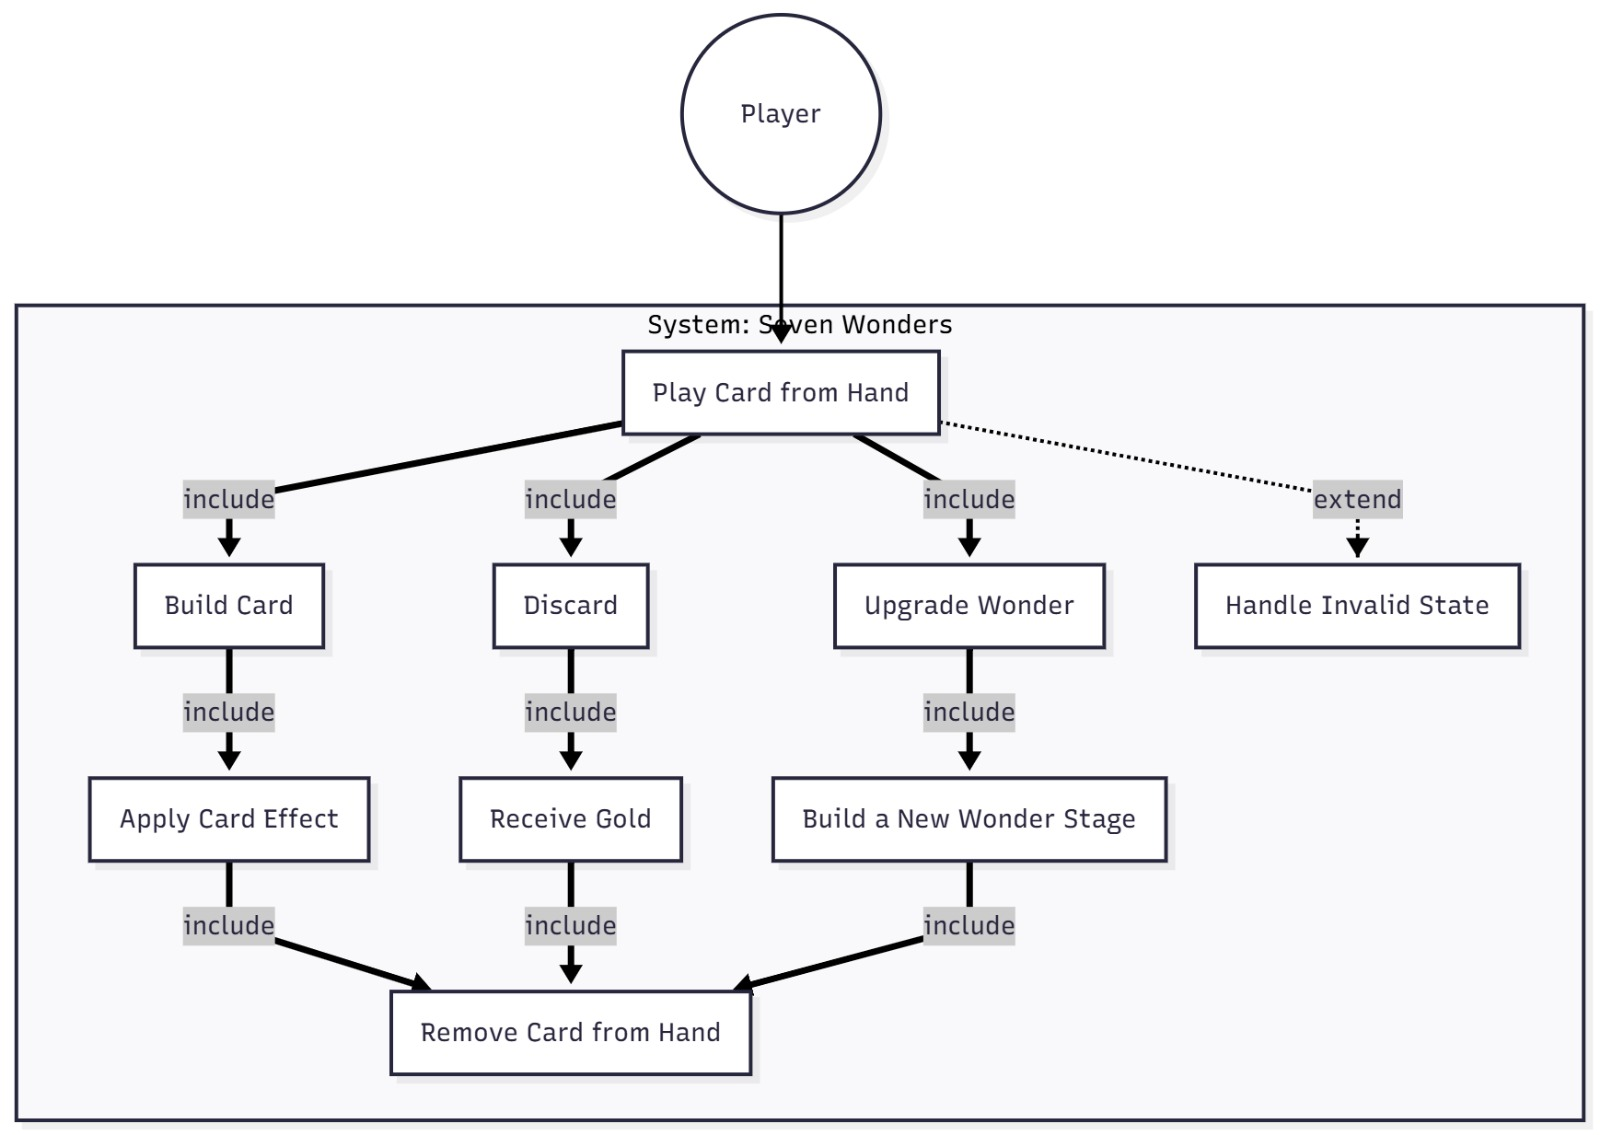
\includegraphics[width=0.6\textwidth]{use_case_0.jpg}
	\caption{Diagramme d'utilisation générale}
	\label{fig:my-screenshot}
\end{figure}
\FloatBarrier

\subsubsection{Scénario 1. Jouer une carte depuis sa main}

\FloatBarrier
\begin{figure}[h]
	\centering
	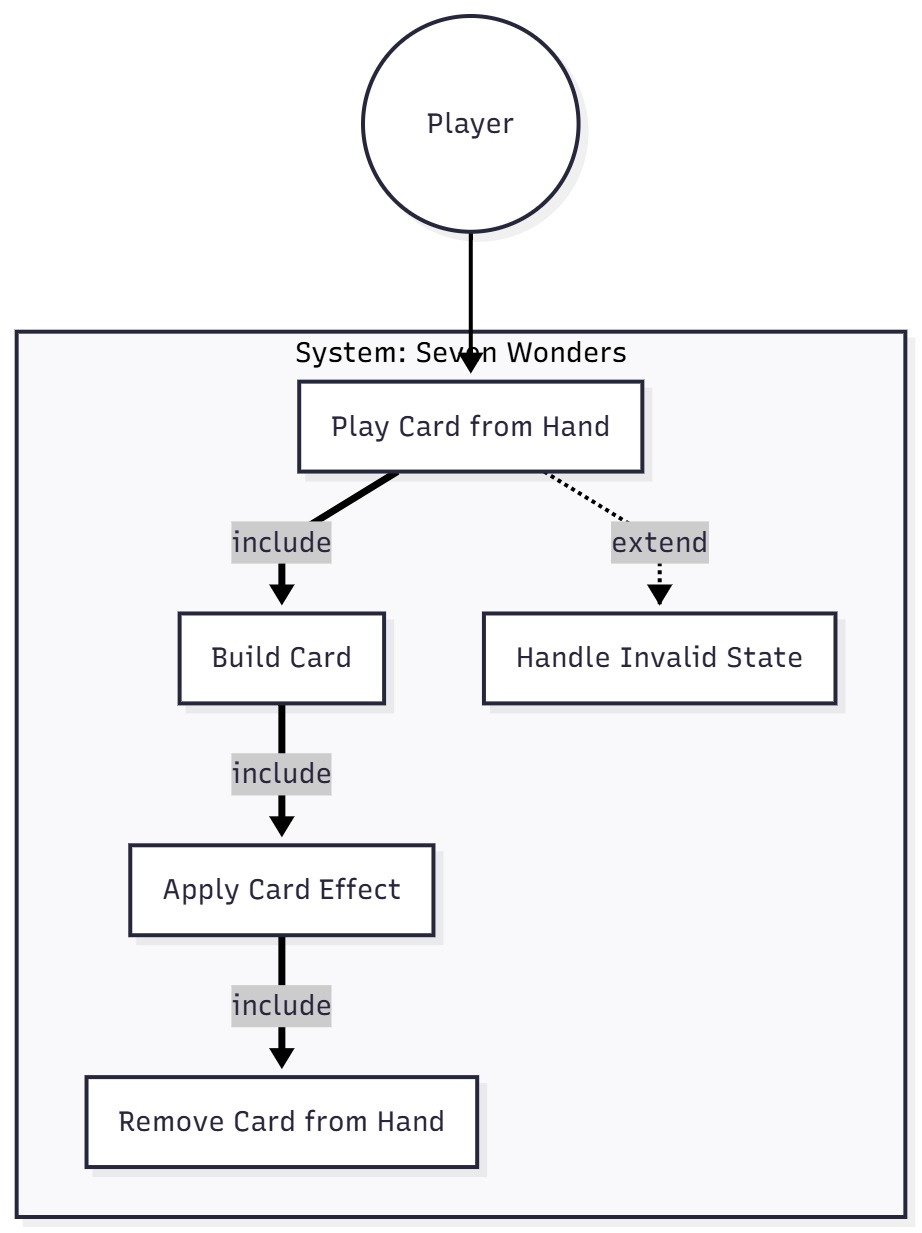
\includegraphics[width=0.4\textwidth]{use_case_1.jpg}
	\caption{Diagramme d'utilisation 1}
	\label{fig:my-screenshot}
\end{figure}
\FloatBarrier

Ce cas d'utilisation décrit le scénario où le Player (Joueur) choisit de jouer une carte pour la construire. L'action principale "Play Card from Hand" inclut l'action "Build Card". Pour être complétée, cette action doit elle-même inclure l'application de l'effet de la carte et le retrait de la carte de la main du joueur. L'ensemble du processus peut être étendu par "Handle Invalid State" pour gérer les cas d'erreur, comme un Out of Bounds exception.

\subsubsection{Scénario 2. Défausser une carte pour de l'or}

\FloatBarrier
\begin{figure}[h]
	\centering
	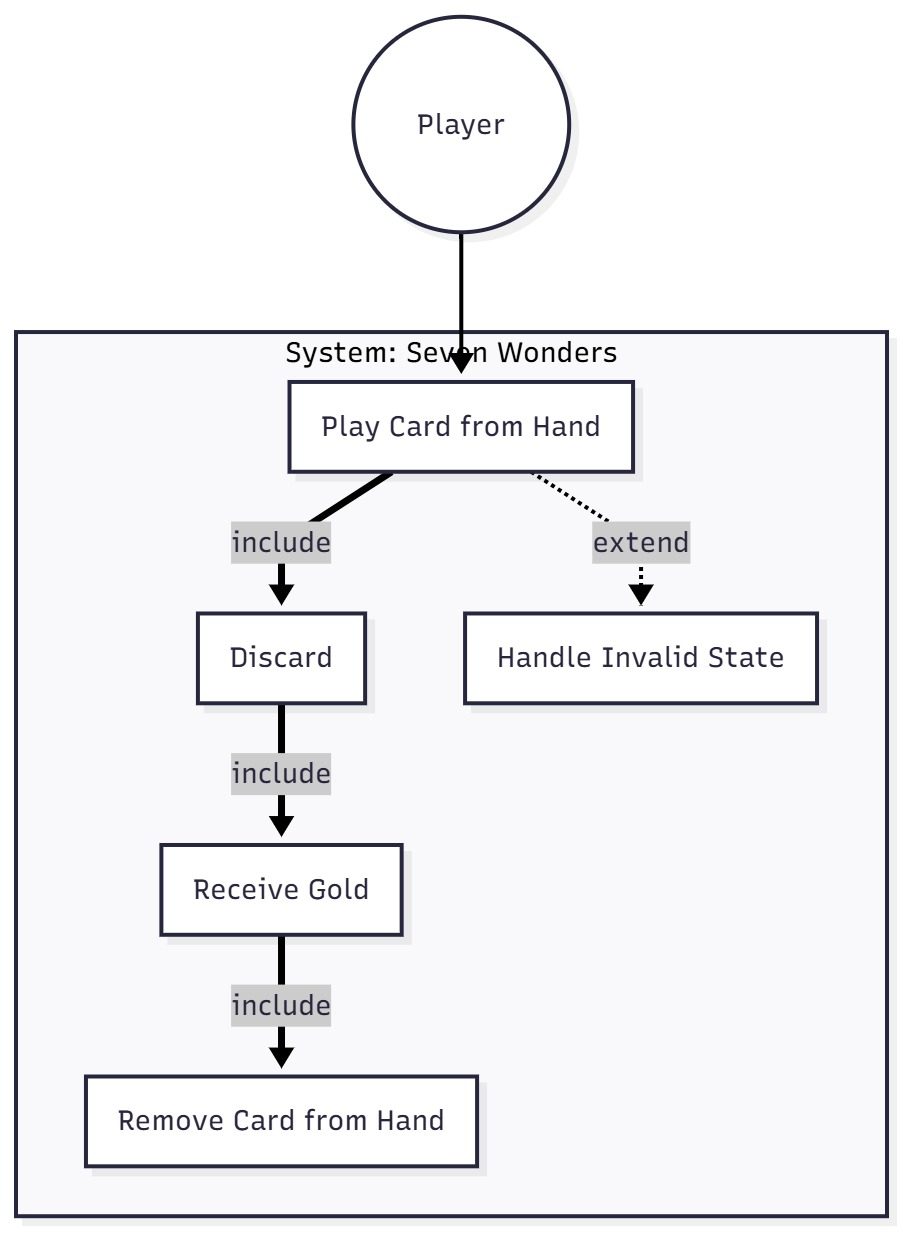
\includegraphics[width=0.6\textwidth]{use_case_2.jpg}
	\caption{Diagramme d'utilisation 2}
	\label{fig:my-screenshot}
\end{figure}
\FloatBarrier

Défausser une carte Ce diagramme illustre le scénario où le Player choisit de défausser une carte pour de l'or. L'action "Play Card from Hand" inclut l'action "Discard". Cette action de défausse entraîne deux sous-actions obligatoires: "Receive Gold" et "Remove Card from Hand". Tout comme les autres cas, ce flux peut être étendu par "Handle Invalid State" si l'action n'est pas valide.

\subsubsection{Scénario 3. Utiliser une carte pour construire une étape de Merveille}

\FloatBarrier
\begin{figure}[h]
	\centering
	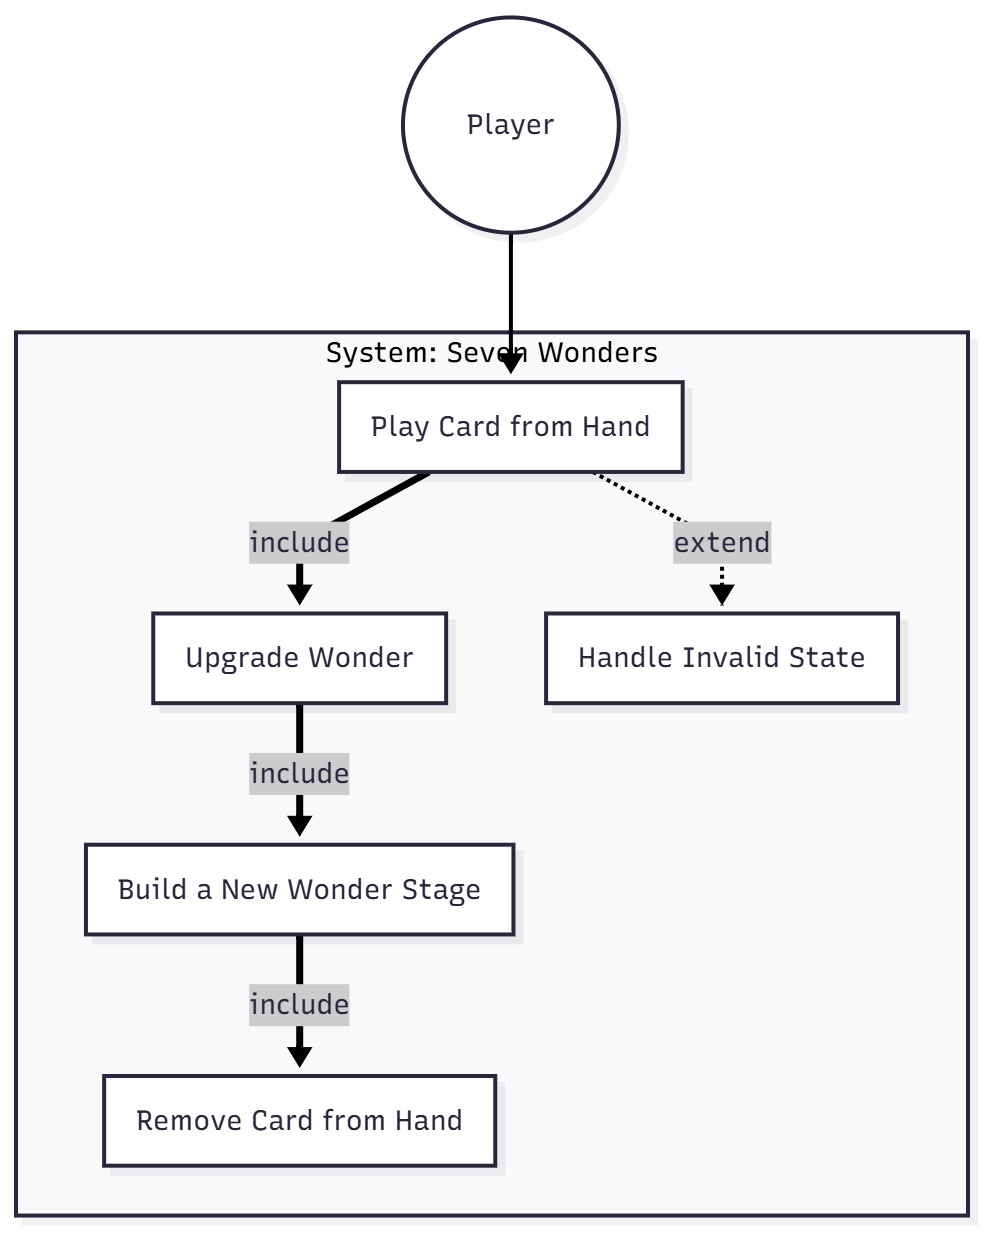
\includegraphics[width=0.6\textwidth]{use_case_3.jpg}
	\caption{Diagramme d'utilisation 3}
	\label{fig:my-screenshot}
\end{figure}
\FloatBarrier

Ce cas d'utilisation montre le flux de construction d'une étape de Merveille. L'action "Play Card from Hand" inclut l'action "Upgrade Wonder". Cette mise à niveau se concrétise par l'inclusion de l'action "Build a New Wonder Stage", qui utilise la carte et la retire de la main. Le cas d'erreur "Handle Invalid State" peut également étendre ce flux.

\section{Conception Logicielle}
\label{conception}

\subsection{Point de vue statique: Diagramme de Classes}

Le point de vue statique de notre application est représenté par le diagramme de classes.

\FloatBarrier
\begin{figure}[h]
	\centering
	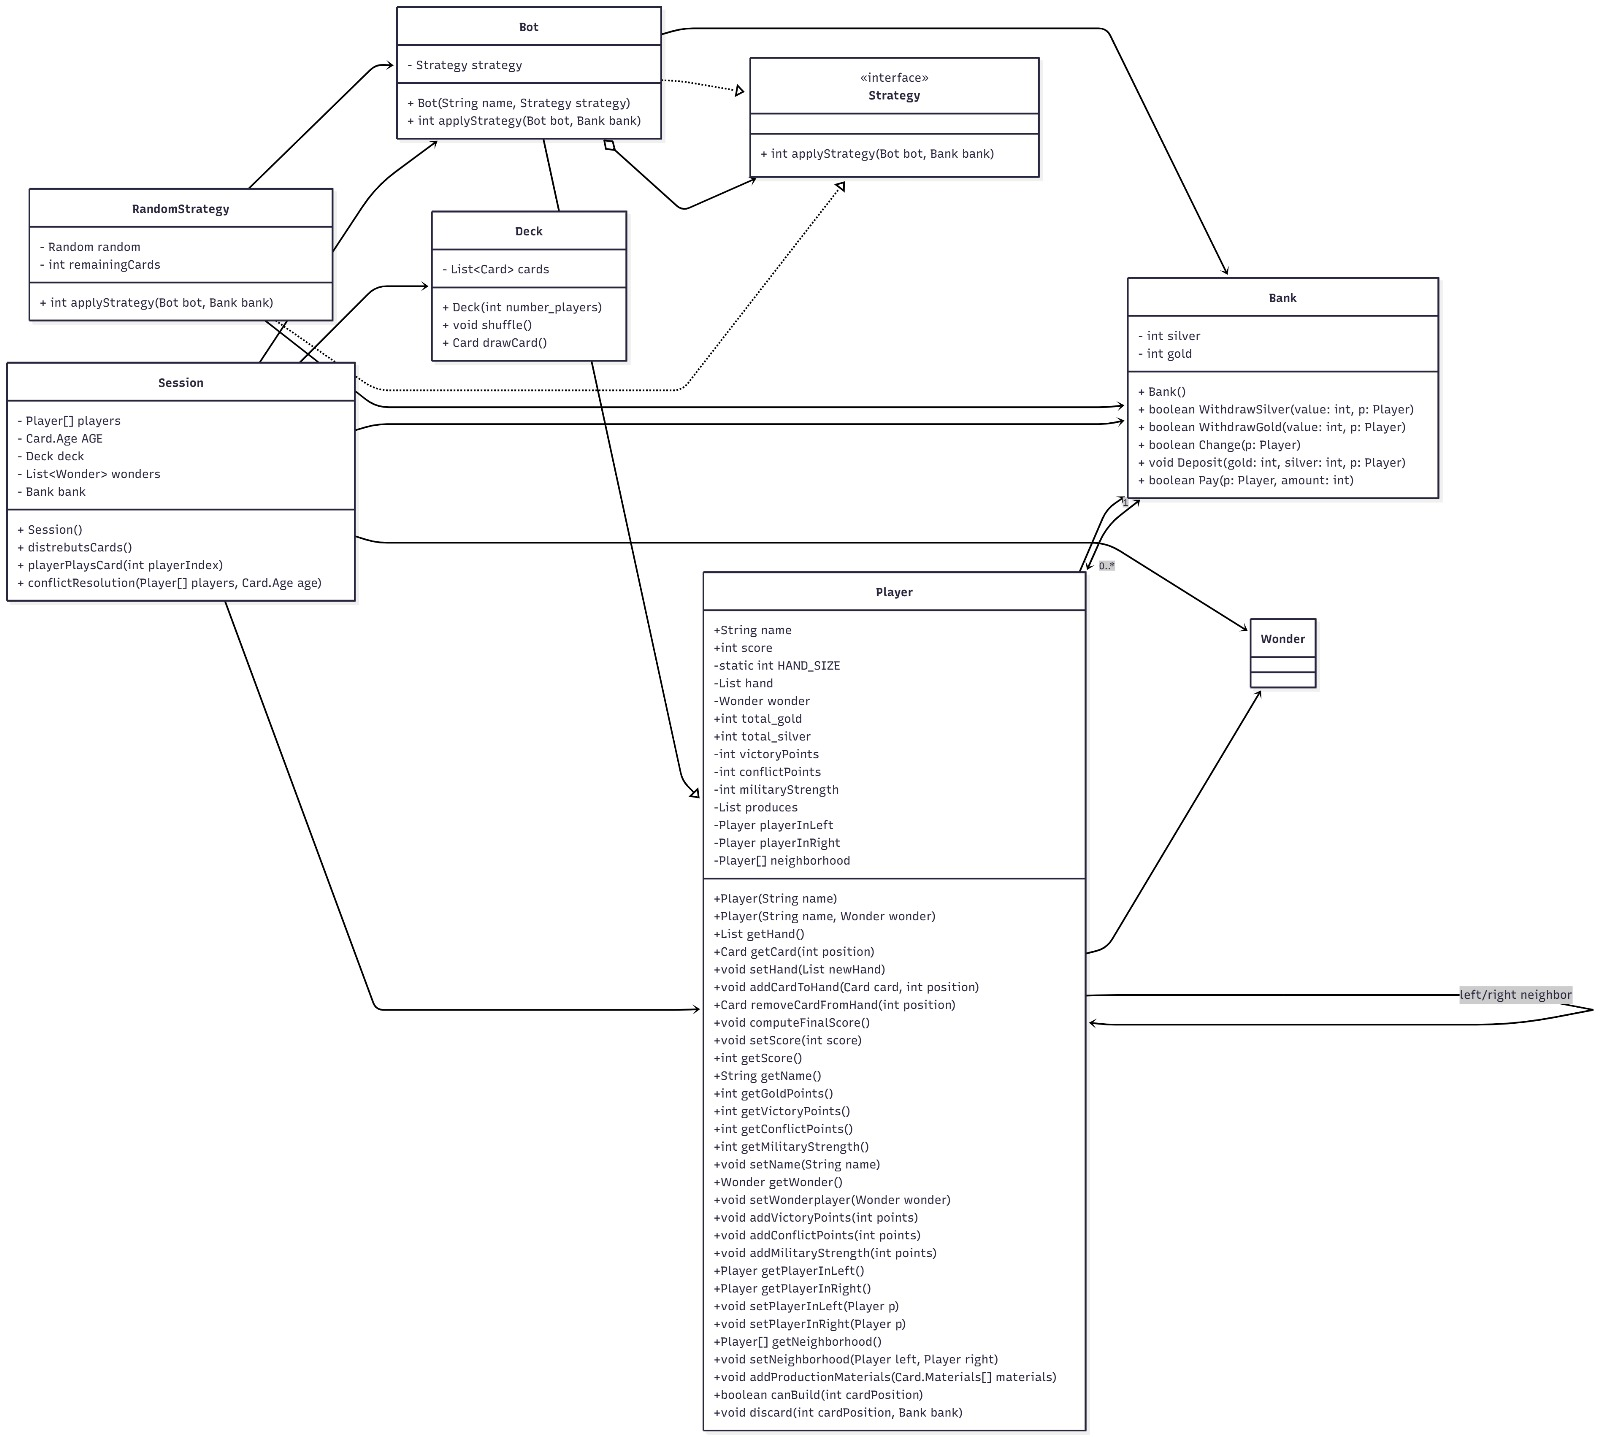
\includegraphics[width=0.8\textwidth]{classe_1.jpg}
	\caption{Diagramme de classes: Score}
	\label{fig:my-screenshot}
\end{figure}
\FloatBarrier

\FloatBarrier
\begin{figure}[h]
	\centering
	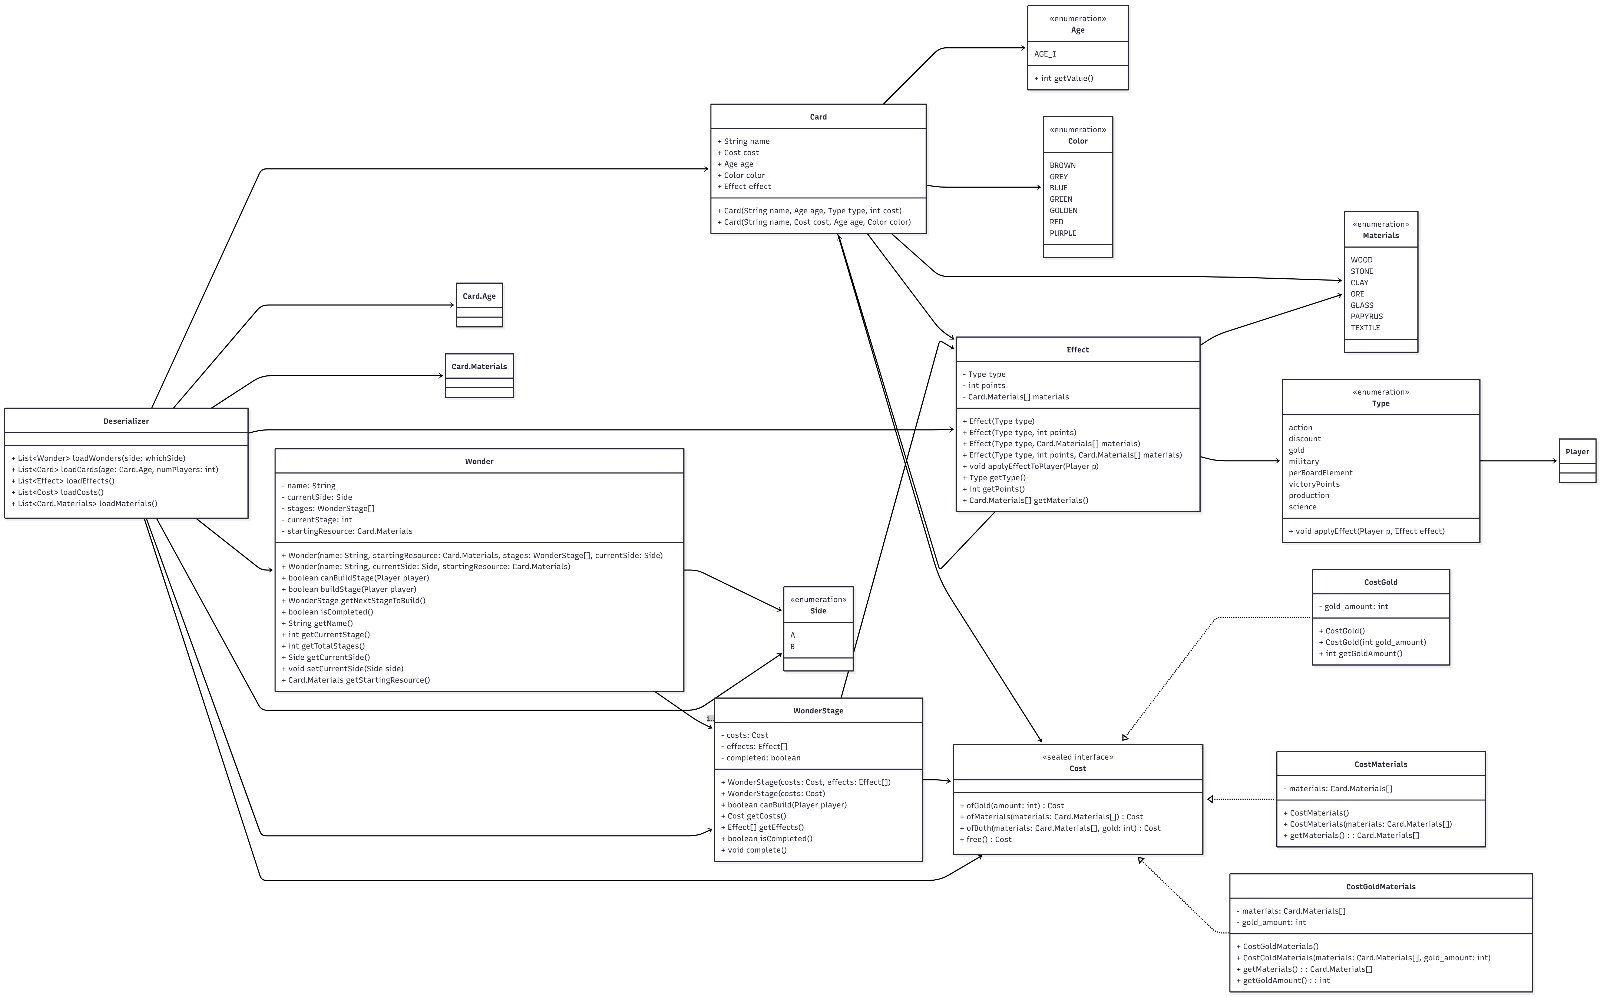
\includegraphics[width=0.8\textwidth]{classe_2.jpg}
	\caption{Diagramme de classes: Models}
	\label{fig:my-screenshot}
\end{figure}
\FloatBarrier

Le cœur du système repose sur la classe Player, qui encapsule l'état d'un joueur : ses ressources (e.g. total\_gold), ses points (e.g. victoryPoints, conflictPoints), sa main de cartes (hand) et sa Merveille (wonder). Les classes Card, Wonder et WonderStage impliquées modélisent respectivement les cartes jouables, le plateau Merveille et ses différentes étapes de construction.

La logique des cartes, notamment la gestion des coûts et des effets, est abstraite via les interfaces Cost et Effect (référencées par Card.java). Cette conception permet d’implémenter différentes variantes de comportement sans modifier la structure du code.

La classe Session agit comme le moteur de jeu. Elle orchestre les interactions entre les joueurs, gère le déroulement des tours (distributeCards, playerPlaysCard), la résolution des conflits militaires (conflictResolution) et le mécanisme de circulation des mains entre voisins (tradeHands). Pour les joueurs automatisés, Session s'adresse aux instances de Bot. Celles-ci, conformément au design pattern Strategy, délèguent la prise de décision à une implémentation de l'interface Strategy (telle que RandomStrategy).

Enfin, les classes de service Deck et Bank gèrent respectivement la distribution des cartes et les ressources monétaires (gold et silver). La classe utilitaire Deserializer prend en charge le chargement des données de jeu (les cartes) depuis des fichiers JSON. La classe Main sert de point d'entrée au programme : elle initialise la Session, puis lui délègue l'exécution de la boucle de jeu principale.

\subsection{Les Patrons de Conception}
\label{sec:design-patterns}

Plusieurs patrons de conception ont été utilisés afin de rendre l’architecture du projet plus robuste, modulaire et extensible.

Le patron Strategy est employé pour la gestion des comportements des bots. Les classes Bot et BotRandom sont des exemples concrets : la classe abstraite Bot définit l’interface commune de prise de décision, tandis que BotRandom implémente une stratégie aléatoire spécifique. Ce patron permettrait d’introduire facilement de nouvelles intelligences artificielles, comme par exemple un BotHeuristique, sans altérer le moteur de jeu.

Le patron Composite est utilisé dans la gestion des effets de cartes à travers l’interface Effect, qui peut regrouper plusieurs effets élémentaires (gain de points, production de ressources, amélioration militaire, etc.) en un seul effet complexe. Ce mécanisme rend la combinaison et l’extension d’effets beaucoup plus flexibles.

Le patron Singleton est appliqué aux classes Bank, Session et Deserializer afin de garantir qu’il n’existe qu’une seule instance de chacune.

Enfin, le patron Observer est partiellement utilisé pour notifier certains changements d’état dans la session, notamment en ce qui concerne les conflits militaires et le passage des cartes entre joueurs.

L’emploi combiné de ces patrons permet de structurer un code flexible, évolutif et conforme aux bonnes pratiques de conception orientée objet, tout en facilitant l’ajout de nouvelles fonctionnalités sans refactorisation majeure.

\subsection{Point de vue dynamique: Diagrammes de Séquence}
\label{sec:diagram-sequence}

\subsubsection{Séquence 1. Jouer une carte depuis sa main}

\FloatBarrier
\begin{figure}[h]
	\centering
	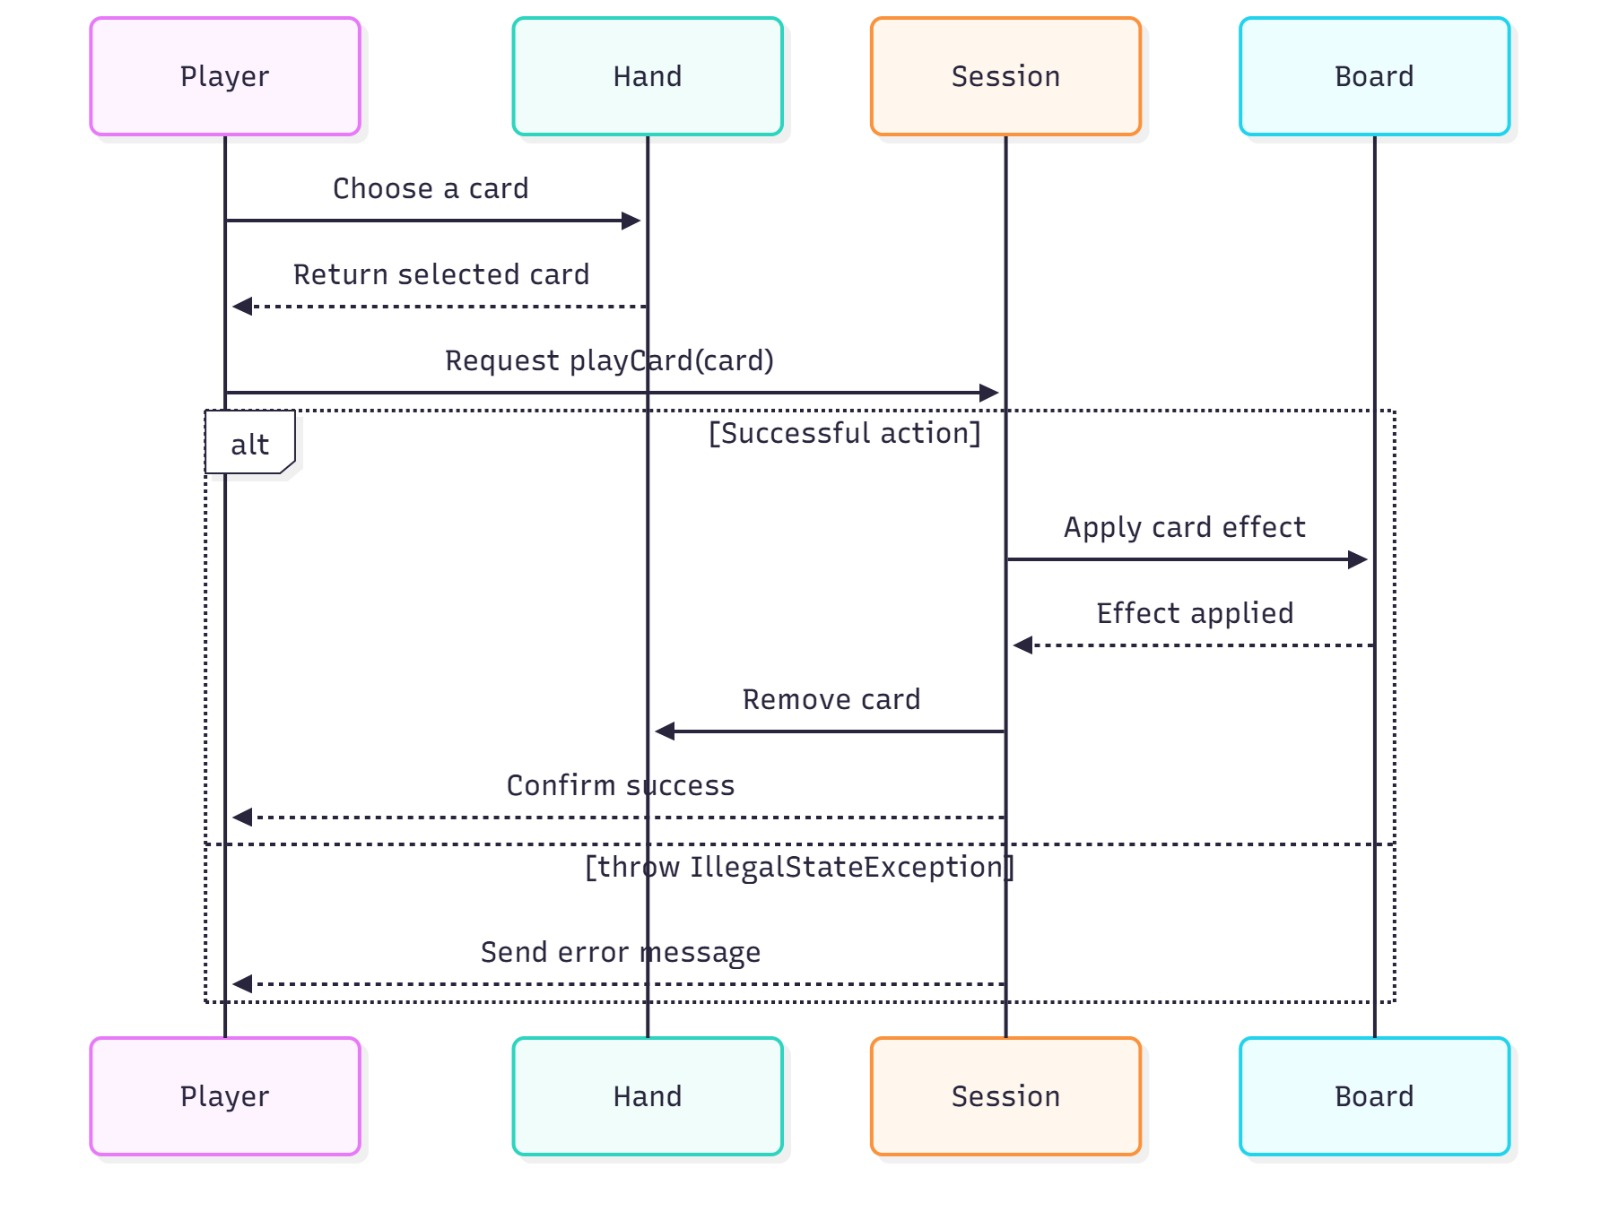
\includegraphics[width=0.5\textwidth]{sequence_1.jpg}
	\caption{Diagramme de sequence 1}
	\label{fig:my-screenshot}
\end{figure}
\FloatBarrier

Le premier diagramme détaille le scénario "Jouer une carte depuis sa main". Le Player sélectionne une carte de sa main et envoie un message playersPlayCard(card) à la Session. La Session, qui agit comme l'orchestrateur ou le moteur de jeu, envoie un message Apply card effect au joueur lui-même. Si l'action réussit (bloc alt), la Session commande à la Player.hand de retirer la carte. En cas d'échec (par exemple, ressources insuffisantes), une exception IllegalStateException est levée.

\subsubsection{Séquence 2. Défausser une carte pour de l'or}

\FloatBarrier
\begin{figure}[h]
	\centering
	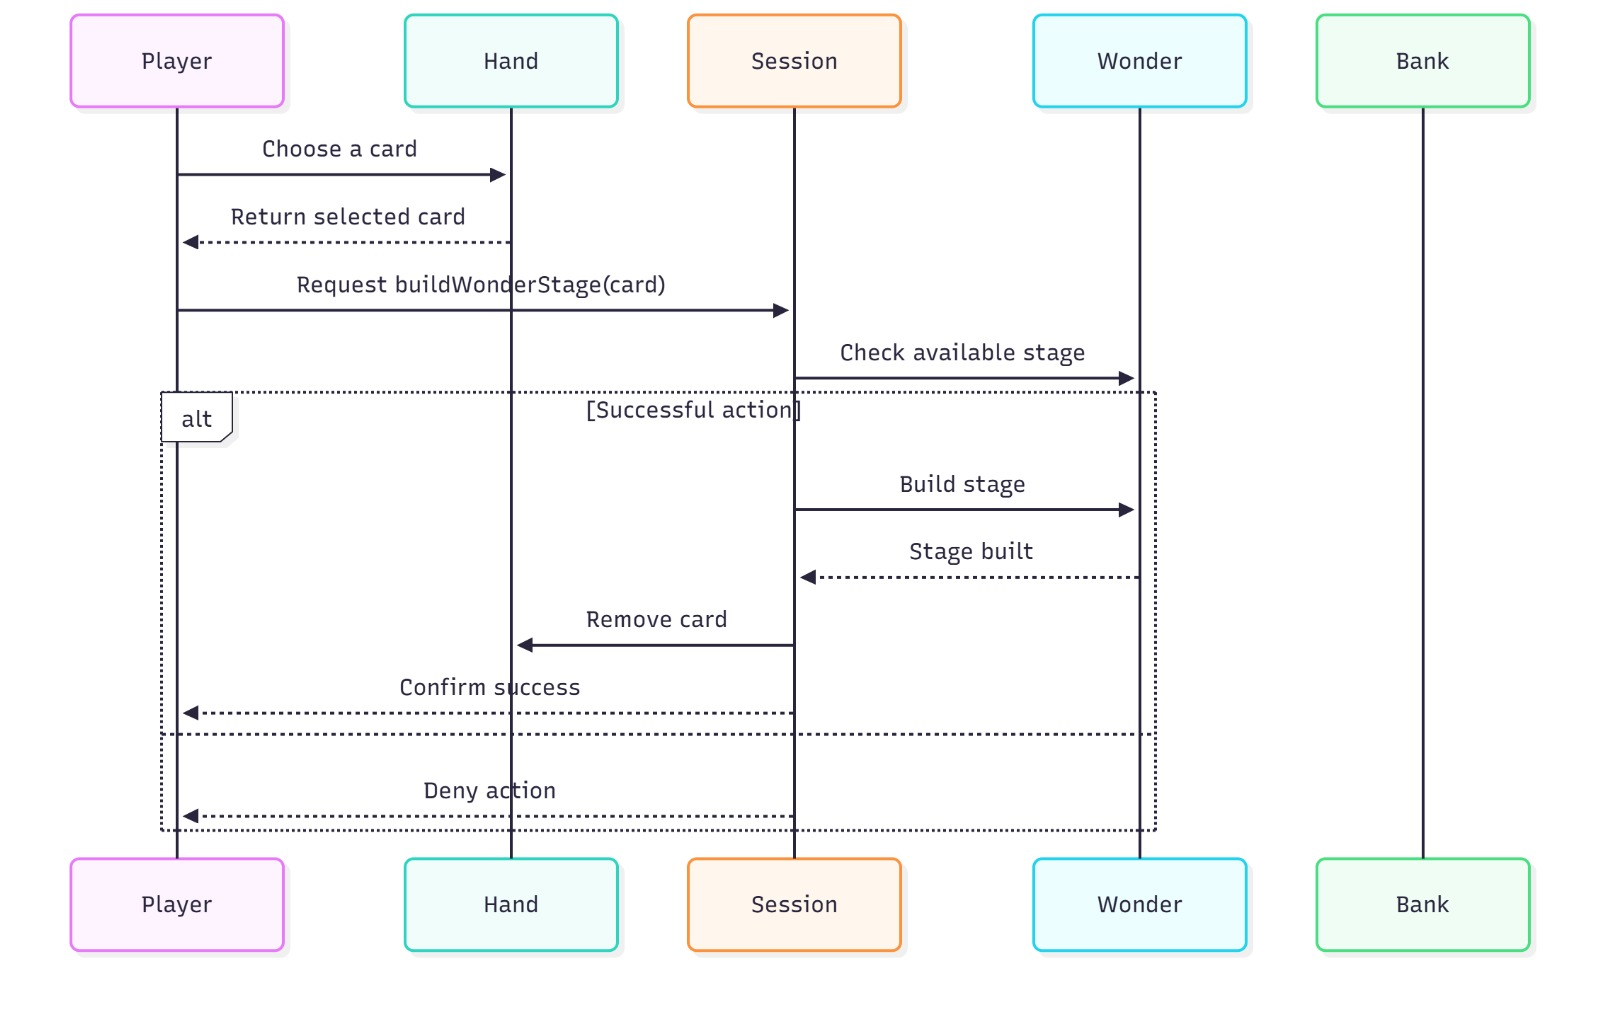
\includegraphics[width=0.8\textwidth]{sequence_2.jpg}
	\caption{Diagramme de sequence 2}
	\label{fig:my-screenshot}
\end{figure}
\FloatBarrier

Le deuxième diagramme correspond au scénario "Défausser une carte pour de l'or". Le Player initie l'action en appelant Player.discard(card) sur la Session. Celle-ci envoie un message à la Bank pour créditer 3 pièces d'or au Player. La Session commande ensuite à la Player.hand de retirer la carte défaussée. Ce flux inclut également un bloc alt pour la gestion des erreurs.

\subsubsection{Séquence 3. Utiliser une carte pour construire une étape de Merveille}

\FloatBarrier
\begin{figure}[h]
	\centering
	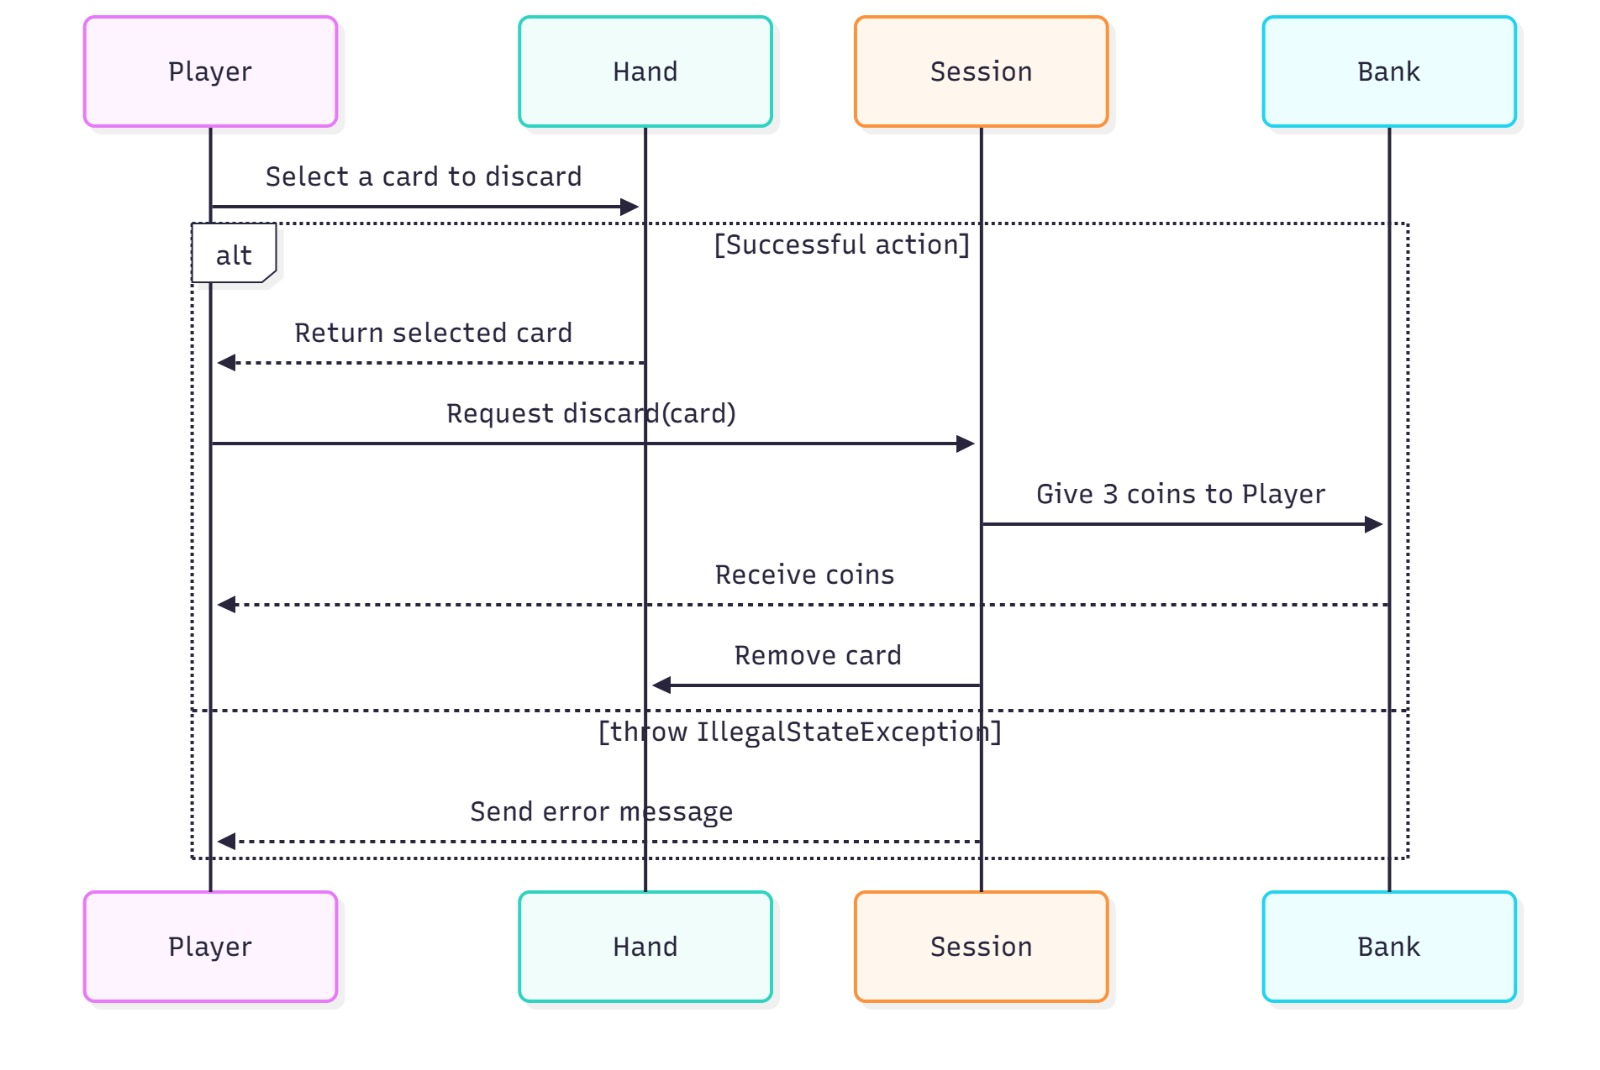
\includegraphics[width=0.8\textwidth]{sequence_3.jpg}
	\caption{Diagramme de sequence 3}
	\label{fig:my-screenshot}
\end{figure}
\FloatBarrier

Le troisième diagramme illustre le scénario "Utiliser une carte pour construire une étape de Merveille". Le Player appelle Wonder.buildWonderStage(card) sur la Session. La Session vérifie d'abord auprès de l'objet Wonder s'il y a une étape disponible. Si l'action est possible (bloc alt), la Session envoie le message Build stage à la Wonder, puis demande à la Hand de retirer la carte utilisée pour la construction.

\section{Conclusion}
\label{sec:conclusion}

La conclusion de ce projet vise à présenter une analyse de la solution mise en œuvre pour le jeu 7 Wonders, en mettant en avant ses forces et ses axes d’amélioration.

\subsection{Points Forts}

Le principal atout de notre solution réside dans la robustesse de sa conception.
L’architecture du projet repose sur une séparation claire des responsabilités entre les différentes classes, ce qui favorise la maintenabilité et la compréhension du code. Le moteur de jeu, incarné par la classe Session, centralise la logique principale tout en déléguant les comportements spécifiques à des entités spécialisées comme Player, Bank ou Bot. Cette modularité facilite l’évolution future du projet, notamment l’ajout de nouveaux Âges, de nouvelles cartes ou de stratégies d’intelligence artificielle plus complexes.

Par ailleurs, l’intégration d’une suite de tests unitaires et d’intégration, combinée à un processus d’intégration continue, garantit la fiabilité du code et facilite la détection rapide d’éventuelles régressions. L’ensemble de ces éléments confère à notre projet une base solide, prête à accueillir de futures évolutions.

\subsection{Points Faibles}

Malgré sa solidité, notre solution demeure incomplète à ce stade du développement. Certaines fonctionnalités clés du jeu 7 Wonders n’ont pas encore été intégrées, notamment les mécanismes avancés de commerce entre voisins, la gestion complète des ressources et la progression des Âges II et III. Le moteur de jeu fonctionne pour une simulation simple, mais il reste des aspects importants du jeu à intégrer pour atteindre une version fidèle à l'original.

De plus, le projet n’exploite pas encore tout le potentiel des patrons de conception disponibles. Une utilisation plus systématique de modèles tels que Observer ou State aurait permis d’améliorer la modularité et de mieux séparer les différents comportements dynamiques du système.

\section{Bilan d'Organisation}
\label{sec:bilan}

Cette section dresse un bilan sur la manière dont le travail a été structuré et géré au cours du développement du projet, aussi bien sur le plan organisationnel que technique.

\subsection{Découpage en Itérations et Gestion des User Stories}
\label{sec:user-story}

Le découpage fonctionnel a été réalisé à partir de User Stories, inspirées de la méthodologie Agile. Chaque User Story décrivait une action du point de vue du joueur ou du système, permettant de relier directement les besoins utilisateurs aux tâches techniques à implémenter. Cette approche a non seulement facilité la planification, mais elle a également permis de prioriser efficacement le travail et de maintenir une vision claire de la progression du projet.

Une particularité importante de notre organisation réside dans le fait que chaque User Story correspondait à une issue GitHub distincte. Cette association directe entre les besoins fonctionnels et les tickets de suivi a grandement simplifié la gestion du développement. Chaque issue décrivait les objectifs et parfois les tâches associées, garantissant une traçabilité entre la conception et la mise en œuvre. Grâce à cette pratique, l’équipe a pu suivre précisément l’avancement du projet, répartir les responsabilités de façon efficace et faciliter la revue de code lors des intégrations successives.

\subsection{Dépôt de Code et Intégration Continue}
\label{sec:repository}

Le dépôt du code a été organisé sur GitHub selon le modèle Git Flow, garantissant une gestion claire des versions et un flux de travail maîtrisé. La branche principale main contient les versions stables, tandis que la branche develop centralise les développements validés au cours de la semaine. Pour chaque nouvelle fonctionnalité, une branche spécifique est créée, puis fusionnée dans develop après validation des tests. Une fois par semaine, à l’issue de chaque livrable, develop est mergé dans main afin de produire un livrable stable et documenté.

Toutes les branches suivent la convention de nommage Conventional Commits, assurant une homogénéité et une lisibilité accrue du code source. Par exemple, une branche peut être nommée feat/add-bank-module pour une nouvelle fonctionnalité, ou fix/update-session-logic pour une correction. L’ensemble des commits respecte cette convention, facilitant la génération automatique de journaux de changements et la relecture des contributions.

\FloatBarrier
\begin{figure}[h]
	\centering
	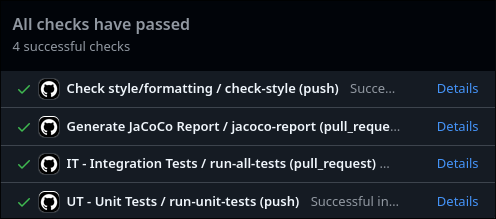
\includegraphics[width=0.8\textwidth]{Screenshot-Github.png}
	\caption{GitHub Actions workflow}
	\label{fig:my-screenshot}
\end{figure}
\FloatBarrier

Le projet intègre également un système d’intégration continue à l’aide de GitHub Actions. Quatre workflows automatisés sont exécutés à chaque modification du code : le premier exécute les tests unitaires, le second les tests d’intégration lors des pull requests, le troisième vérifie le style du code à l’aide de mvn spotless:check, et le dernier génère les rapports de couverture JaCoCo. Ces actions automatisées garantissent la qualité du code, réduisent les erreurs humaines et assurent la cohérence des livraisons hebdomadaires.

Enfin, une politique linguistique a été définie afin d’équilibrer rigueur technique et accessibilité. Le code, les noms de branches et les messages de commit sont rédigés en anglais, conformément aux standards du développement international. En revanche, les issues, les descriptions des pull requests et la documentation du dépôt sont rédigées en français, afin de favoriser la clarté pour l'évaluation par l'enseignant.

	
%Working with LaTeX - EXAMPLE
%\input{90_latex}

%insert further chapters here
%\input{03_neues_kapitel}

%Glossary
\clearpage
\renewcommand{\sectionmark}[1]{\markboth{#1}{}}

\section*{Glossaire}
\addcontentsline{toc}{section}{Glossaire}
\label{sec:glossaire}
\sectionmark{Glossaire et Abréviations}

\noindent 
\textit{Abréviations}

\vspace{6pt}

\noindent 
\begin{tabular}{@{}p{4cm}l}
	CI&Intégration Continue (Continuous Integration)\\
	IT&Test d'Intégration (Integration Test)\\
	JSON&JavaScript Object Notation\\
	PR&Pull Request (Demande de fusion)\\
	UT&Test Unitaire (Unit Test)\\
\end{tabular}

\vspace{18pt}

\noindent 
\textit{Technologies et Outils}

\vspace{6pt}

\noindent 
\begin{tabular}{@{}p{4cm}l}
	Git Flow&Modèle de gestion des branches pour Git\\
	GitHub&Plateforme d'hébergement de code et de gestion de projet\\
	GitHub Actions&Outil d'intégration continue intégré à GitHub\\
	JaCoCo&Outil de mesure de la couverture de code pour Java\\
	JavaDoc&Générateur de documentation pour le code source Java\\
	JUnit&Framework de test unitaire pour Java\\
	Maven&Outil de gestion de projet et d'automatisation de build\\
	Mockito&Framework de création d'objets simulés (mocks) pour les tests\\
	Spotless&Plugin Maven pour le formatage automatisé du code\\
\end{tabular}

\vspace{18pt}

\noindent 
\textit{Concepts de Conception et Méthodologie}

\vspace{6pt}

\noindent 
\begin{tabular}{@{}p{4cm}l}
	Agile&Méthodologie de développement logiciel itérative\\
	Composite&Patron de conception structurel\\
	Conventional Commits&Convention de nommage pour les messages de commit\\
	Observer&Patron de conception comportemental\\
	Singleton&Patron de conception de création\\
	Strategy&Patron de conception comportemental\\
	User Story&Description d'une fonctionnalité du point de vue de l'utilisateur\\
\end{tabular}

\vspace{18pt}

\noindent 
\textit{Termes Spécifiques au Projet}

\vspace{6pt}

\noindent 
\begin{tabular}{@{}p{4cm}l}
	*IT.java&Suffixe de fichier pour les tests d'intégration\\
	*Test.java&Suffixe de fichier pour les tests unitaires\\
	Âge I&Première phase du jeu 7 Wonders\\
	Bank&Classe gérant les ressources monétaires\\
	Bot&Classe représentant un joueur automatisé (IA)\\
	Deserializer&Classe gérant le chargement des données depuis JSON\\
	Player&Classe encapsulant l'état d'un joueur\\
	Session&Classe agissant comme le moteur central du jeu\\
	Wonder&Classe modélisant le plateau Merveille d'un joueur\\
\end{tabular}

%Bibliography
\clearpage
\printbibliography[heading=bibintoc]

%Appendix
%Detailed data tables, extensive flow charts and long calculations can be put in the appendix
%\clearpage
%\appendix
%\input{99_anhang}

\end{document}
